%----------------------------------------------------------------------------------------
%	PACKAGES AND THEMES
%----------------------------------------------------------------------------------------

\documentclass[presentation,aspectratio=1610]{beamer}

\usetheme{Coventry}
\graphicspath{{./picture/}}

%----------------------------------------------------------------------------------------
%	TITLE PAGE
%----------------------------------------------------------------------------------------

\title[WHURS]{武汉大学遥感信息工程学院 Beamer 模板} % The short title appears at the bottom of every slide, the full title is only on the title page
\subtitle{————这里是副标题}

\author{向征} % Your name
\institute[WHU] % Your institution as it will appear on the bottom of every slide, may be shorthand to save space
{
武汉大学遥感信息工程学院 \\ % Your institution for the title page
\medskip
\textit{hspili@live.com} % Your email address
}
\date{\today} % Date, can be changed to a custom date

\begin{document}

\begin{frame}
\titlepage % Print the title page as the first slide
\end{frame}

\begin{frame}
\frametitle{目录} % Table of contents slide, comment this block out to remove it
\tableofcontents % Throughout your presentation, if you choose to use \section{} and \subsection{} commands, these will automatically be printed on this slide as an overview of your presentation
\end{frame}

%----------------------------------------------------------------------------------------
%	PRESENTATION SLIDES
%----------------------------------------------------------------------------------------

%------------------------------------------------
\section{介绍} % Sections can be created in order to organize your presentation into discrete blocks, all sections and subsections are automatically printed in the table of contents as an overview of the talk
%------------------------------------------------

%\subsection{编译方式} % A subsection can be created just before a set of slides with a common theme to further break down your presentation into chunks

\begin{frame}
\frametitle{介绍}
	\begin{itemize}
	\item 改编自如下Beamer主题:\url{https://github.com/dscroft/coventry_beamer}
    \item {编译方式}
	    \begin{itemize}
	    	\item 推荐安装完整版的 TeXLive
	    	\item 编译方式为:xelatex -> biber -> xelatex*2
	    \end{itemize}
    \item 请参考 \LaTeX 和 Beamer 用户文档 
    \item 内置五种主题颜色(蓝、绿、橙、紫、红),默认采用蓝色
    \item 默认长宽比为16:10,提供16:9与4:3选项对应的背景水印排布方式
  \end{itemize}
\end{frame}

%------------------------------------------------
\section{测试} % Sections can be created in order to organize your presentation into discrete blocks, all sections and subsections are automatically printed in the table of contents as an overview of the talk
%------------------------------------------------

\subsection{分块测试} % A subsection can be created just before a set of slides with a common theme to further break down your presentation into chunks

\begin{frame}
\frametitle{分块测试}
	\begin{block}{分块 1}
	这是第1分块。
	\end{block}

	\begin{block}{Block 2}
	This is the second block.
	\end{block}

	\begin{block}{Block 3}
	A long long time ago in a galaxy far far away...
	\end{block}
\end{frame}

%------------------------------------------------

\subsection{分栏测试}

\begin{frame}
\frametitle{分栏测试}
\begin{columns}[c] % The "c" option specifies centered vertical alignment while the "t" option is used for top vertical alignment

\column{.45\textwidth} % Left column and width
\textbf{Heading}
\begin{enumerate}
\item Statement(陈述)
\item Explanation(解释)
\item Example(示例)
\end{enumerate}

\column{.5\textwidth} % Right column and width
Wuhan University is in Wuhan, Hubei.
It is one of the most prestigious and selective universities in China, which has been selected as a Chinese Ministry of Education Class A Double First Class University.
It was one of the four elite universities in the republican period and also one of the oldest universities in China.

\end{columns}
\end{frame}

%------------------------------------------------

\subsection{表格测试}

\begin{frame}
\frametitle{表格测试}
\begin{table}
\begin{tabular}{l l l}
\toprule
\textbf{Treatments} & \textbf{Response 1} & \textbf{Response 2}\\
\midrule
Treatment 1 & 0.0003262 & 0.562 \\
Treatment 2 & 0.0015681 & 0.910 \\
Treatment 3 & 0.0009271 & 0.296 \\
\bottomrule
\end{tabular}
\caption{测试表格}
\end{table}
\end{frame}

%------------------------------------------------

\subsection{公式测试}

\begin{frame}
\frametitle{公式测试}
Given $ g:[0,∞) \to\mathbb{R} $, With $ g(0)=0 $, derive the formula

\begin{equation}
	u(x,t)=\frac{x}{\sqrt{4\pi}}\int_{0}^{t}\frac{1}{(t-s)^{\frac{3}{2}}}e^{\frac{-x^2}{4(t-s)}}g(s)ds
\end{equation}

for a solution of the initial/boundary value problem 

\[
	\begin{cases}
		u_t-u_{xx}  = 0   & \mbox{in }  \mathbb{R}_+ \times(0,\infty)\\
		u           = 0   & \mbox{on }  \mathbb{R}_+ \times\{t=0\}\\
		u           = g   & \mbox{on }  \{x=0\}\times[0,\infty)
	\end{cases}
\]

(Hint: Let $v(x, t) := u(x, t) − g(t)$ and extend $v$ to $\{x < 0\}$ by odd reflection.)
\end{frame}

%------------------------------------------------

\subsection{代码测试}

\begin{frame}[fragile] % Need to use the fragile option when verbatim is used in the slide
\frametitle{代码测试}
\begin{example}[main.cpp]
\begin{verbatim}
#include<iostream>
using namespace std;
int main(){
    cout<<"Hello World!"<<endl;
    return 0;
}
\end{verbatim}
\end{example}
\end{frame}

%------------------------------------------------

\subsection{图片测试}

\begin{frame}
\frametitle{图片测试}
\begin{figure}
	\begin{subfigure}{0.45\textwidth}
	  \centering
	  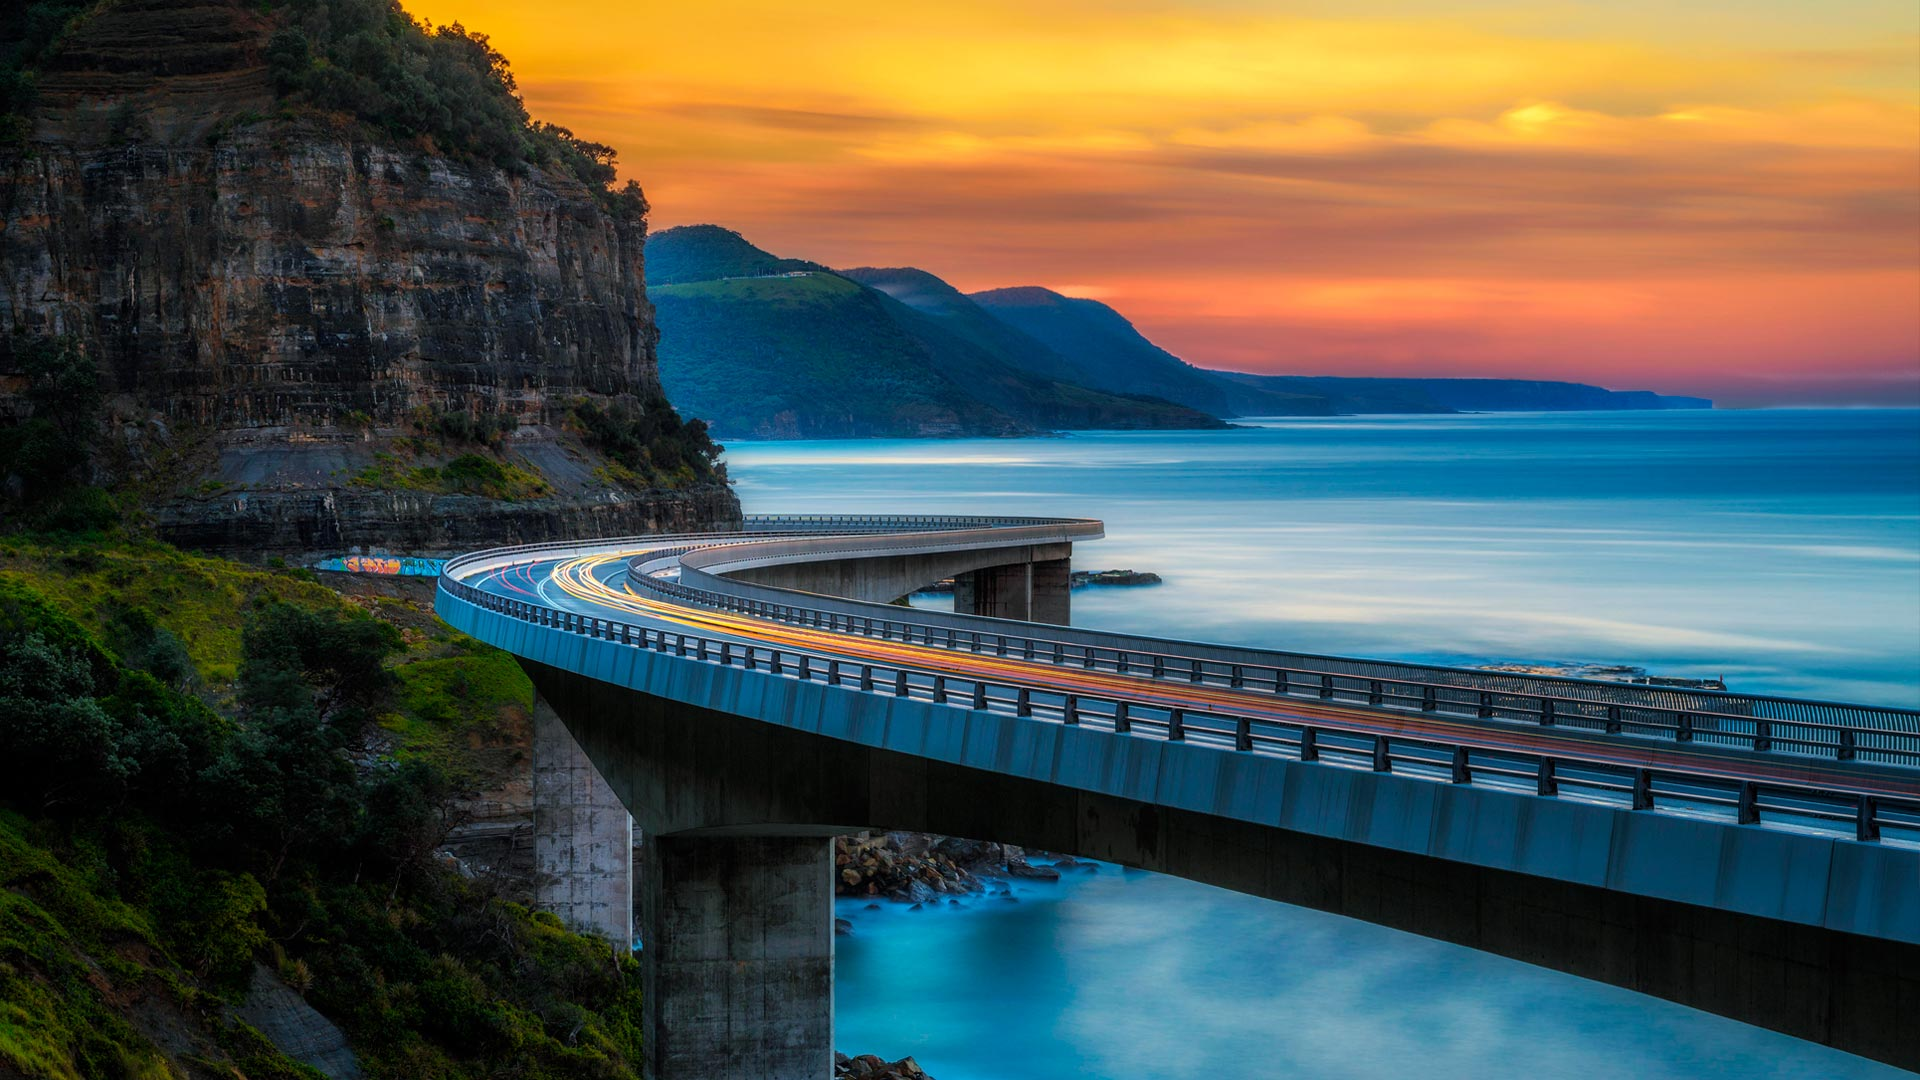
\includegraphics[width=0.8\linewidth]{image1.jpg}
	  \caption{1a}
	  \label{fig:sfig1}
	\end{subfigure}%
	\begin{subfigure}{0.45\textwidth}
	  \centering
	  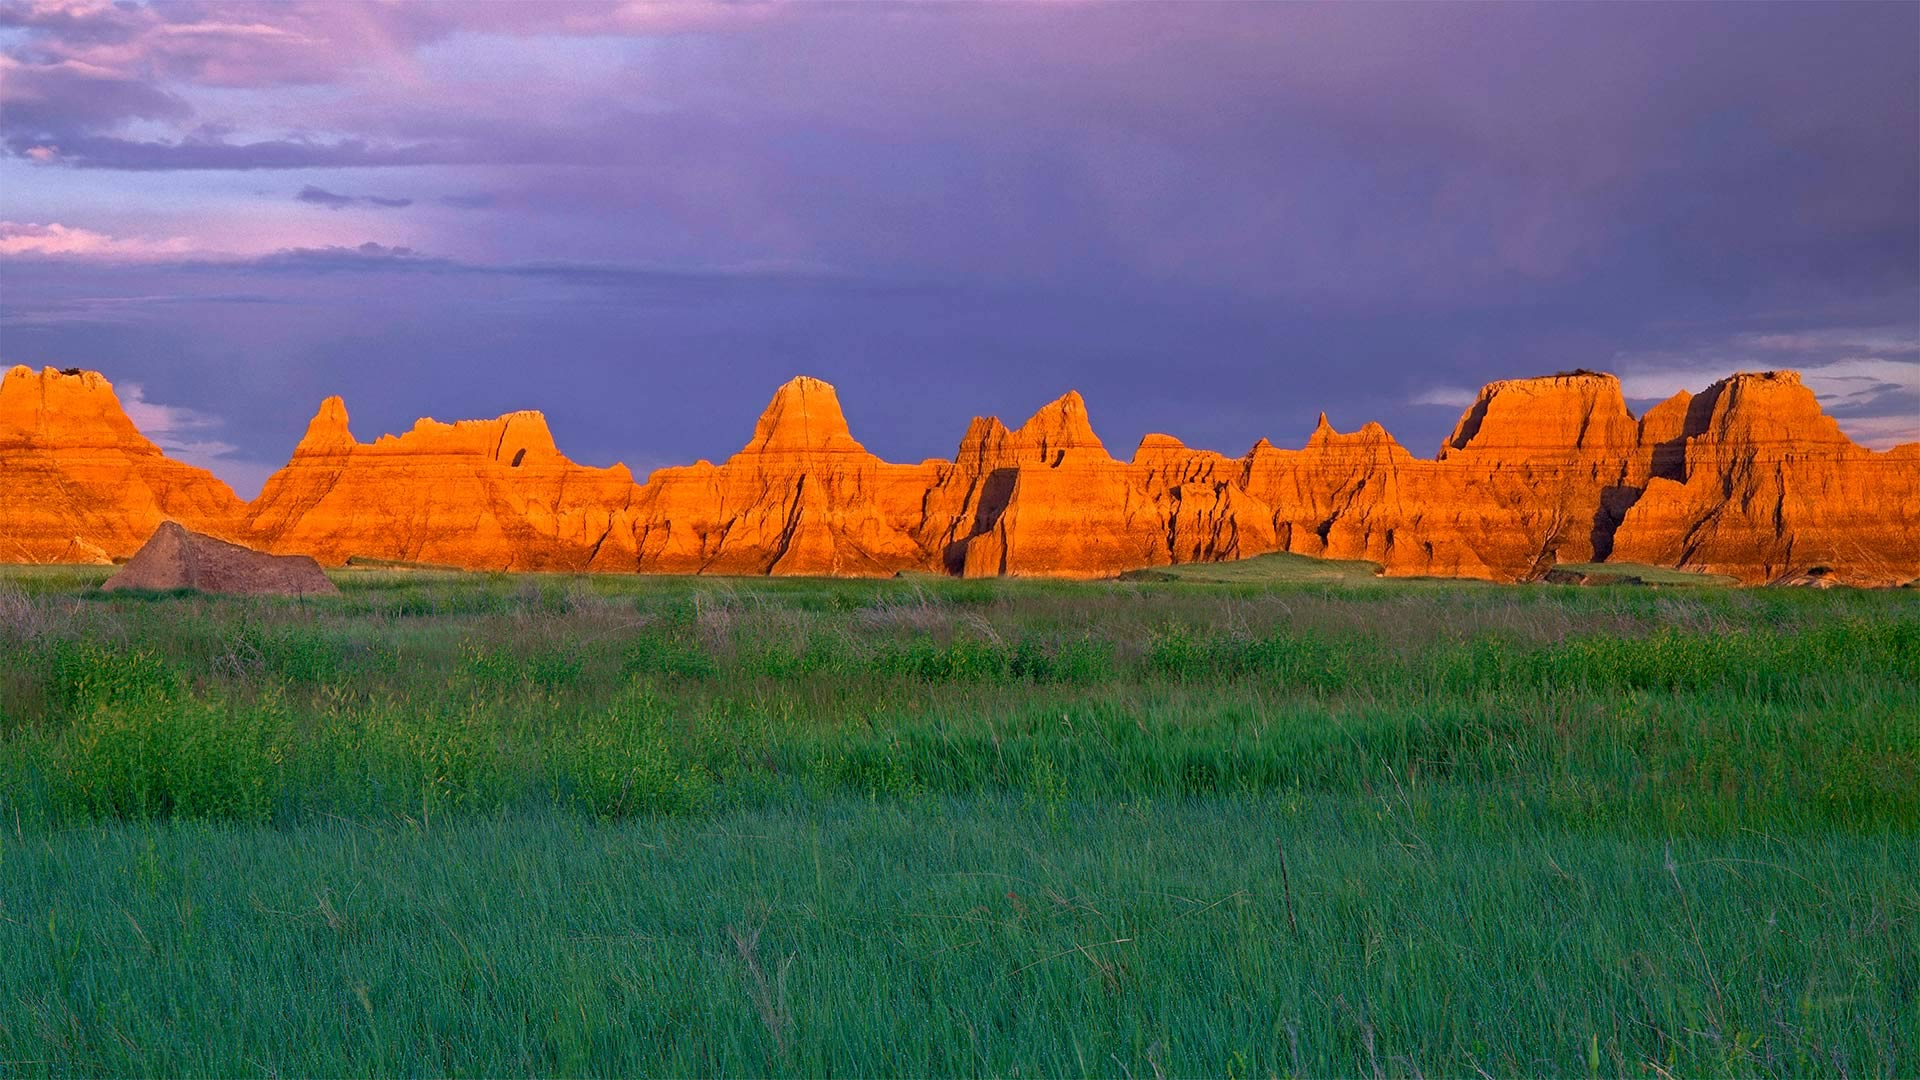
\includegraphics[width=0.8\linewidth]{image2.jpg}
	  \caption{1b}
	  \label{fig:sfig2}
	\end{subfigure}
	\caption{测试图像}
	\label{fig:fig}
	\end{figure}
\end{frame}

%------------------------------------------------

\subsection{引用测试}
  
\begin{frame}[t,allowframebreaks]
	\frametitle{参考文献}
	\nocite{*}
	\printbibliography
\end{frame}

%------------------------------------------------

\section{}

\begin{frame}{}
	\centering
		\Huge\bfseries
	\textcolor{whucolor}{The End}
\end{frame}

%----------------------------------------------------------------------------------------

\end{document}
